\documentclass[ngerman,11pt,parskip=half] {scrartcl}

\usepackage{babel}

%
% Schrift
%
\usepackage[T1]{fontenc}
\usepackage{textcomp}
\usepackage[utf8]{inputenc}
\usepackage{eurosym}% 1 \euro oder \EUR{1}

\usepackage{helvet}
\renewcommand{\ttdefault}{pcr} %typewriter default font
\renewcommand{\familydefault}{\sfdefault}

%
% Layout
%
\usepackage[textwidth=16cm,head=4cm,bottom=3cm,a4paper]{geometry}
\usepackage{scrpage2}
\pagestyle{scrheadings}
%\chead{}\ihead{}\ohead{}
\cfoot{}\ifoot{\footnotesize \currfilepath}\ofoot{\footnotesize Seite \pagemark~von \pageref*{LastPage}} % pageref* -> kein klickbarer Link
\renewcommand*{\footfont}{\normalfont}%nicht kursiv

\usepackage{lastpage}
\usepackage[table]{xcolor}
\usepackage{multicol}
\usepackage{rotating}
\usepackage{graphicx}
\usepackage{setspace}
\linespread{1.1}%zeilenabstand default global
\usepackage{array}
\usepackage{longtable}
\usepackage{ltxtable}
\setlength\LTleft{0pt}
\setlength\LTright\fill
\usepackage{tikz}
\usepackage{ctable}
\newcommand{\otoprule}{\midrule[\heavyrulewidth]}
\usepackage{hhline}
\usepackage{cals}
\usepackage{enumitem}% f"ur besseres itemize
\setitemize{label=\textminus,itemsep=0pt,topsep=0.5ex,after=\vspace{\baselineskip}}
\usepackage{float} %bilderpositionierung
%\usepackage{textgreek}
\usepackage{sansmath}

% Funktion zum Generieren des Dateipfades. Kann leider nicht den absoluten Pfad finden...
\usepackage{currfile}

% Zeit
\usepackage{datetime}

%
% Funktionen
%
% fettes rotes todo
\newcommand {\todo} {\textbf{\color{red} todo\ }}
% Gr"o"se eines Oszillogramms
\newcommand {\tscopesize}{12cm}

% Links, Querverweise, Titel
\usepackage[
  colorlinks=true,
  linkcolor=black,
  urlcolor=black,
  pdftitle={Schaltungsbeschreibung}, %PDF Beschreibung
  allcolors=black,
]{hyperref} %immer zum Schluss

%
% Dokument
%
\begin{document}
\sansmath

% Titelseite

\thispagestyle{empty}

\mbox{}\\[2cm]%absolute L"ange

\textbf{\huge
Saba Webradio Hardware
}

\vfill

\hspace{1cm}\begin{tabular}{ll}
Autor: & 		Martin Wagner, DL2WAG\\
Dokumentart:&   Schaltungsbeschreibung, Messungen\\
Datum:&         \today \enspace \currenttime
\end{tabular}




\vfill
\begin{minipage}[t]{\textwidth}
\begin{spacing}{1.2}%zeilenabstand lokal 
  \begin{tabular}{p{.1\textwidth} p{.2\textwidth}  p{.6\textwidth}}%
  Version & Datum & Bemerkung        \\
  \hline  
  \hspace{.02\textwidth} 1  & 09.04.2021 & Neu   \\  
  \end{tabular}
\end{spacing}
\end{minipage}


\mbox{}\\[2cm]%absolute L"ange

% Inhaltsverzeichnis

\newpage
\tableofcontents

% eigentliches Dokument

\newpage

\section{Saba Webradio} \label{sec:sabawebradio}

Das Saba Webradio erweitert ein Saba Automatic Radio um die folgenden Funktionen:
\begin{itemize}
\item WLan Webradio (hence the name)
\item Steuerung von Automatik und Lautst"arke per Webinterface, MQTT, IR Fernbedienung ...
\item Steuerung des Webradio per Radio Automatiktasten
\end{itemize}
Es kann direkt auf die Anschlussbuchse f"ur die Fernbedienung aufgesteckt werden. Kompatibel sind mind. das Meersburg und Freiburg 6-3D. Am Ger"at selbst sind keine Modifikationen notwendig (aber empfehlen). Der Audioausgang des Webradio wird mit dem TA Eingang des Radios verbunden und kann durch Wahl des zugeh"origen Eingangs am Radio verwendet werden.

\todo Bild Stecker mit Ma"sen.

Das Webradio basiert auf dem \emph{\href{https://github.com/Edzelf/ESP32-Radio}{ESP32-Radio Projekt von Ed Smallenburg}}.

\todo github link radio hw und modifizierte sw


\section{Empfohlene Modifikationen} \label{sec:mod}

Wird h"aufig die Webradiofunktion verwendet, sollte das magische Auge im TA Betrieb deaktiviert werden. Bei neueren Saba Ger"aten ist dies ab Werk der Fall, bei "alteren wie dem 6-3D wie folgt modifizieren:

\begin{figure}[H]
\centering
\begin{tikzpicture}
     \node[anchor=south west,inner sep=0] at (0,0) {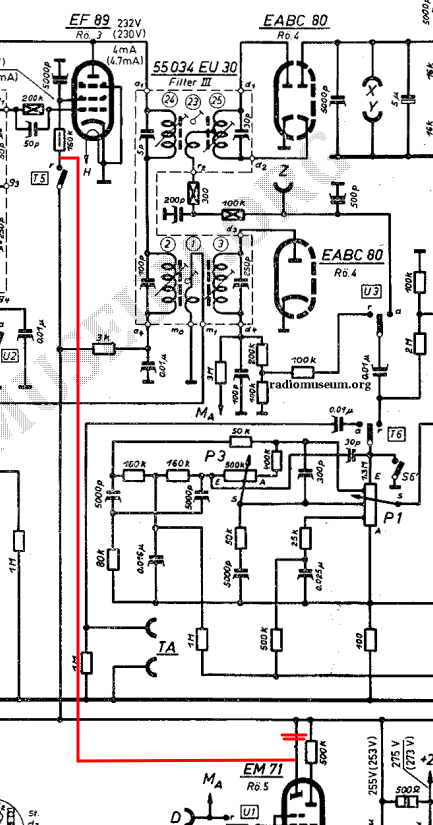
\includegraphics[width=6cm]{auge.png}};
\end{tikzpicture}
\caption{Schaltungsvorschlag } \label{fig:1}
\end{figure}

\section{Bedienung} \label{sec:bedienung}

\todo

\section{Schaltungsbeschreibung} \label{sec:schaltung}

Die Schaltung besteht aus folgenden Bl"ocken:
\begin{itemize}
\item Microcontroller ESP32 auf Daughterboard
\item Audioschaltung
\item Radio steuern per Webradio
\item Webradio steuern per Radio
\item Spannungsversorgung
\item Schnittstellen
\end{itemize}

In den folgenden Kapiteln wird Design, Funktion und Zusammenwirken beschrieben.

\subsection{Datenbl"atter} \label{sec:schaltung:datenblaetter}

Folgende Datenbl"atter und Application Notes wurden verwendet (u.A):
\begin{itemize}
\item ADA4522-1/ADA4522-2/ADA4522-4 Rev. F
\item AD8655/AD8656 Rev. E
\item VS1053b Datasheet Version: 1.31, 2017-11-17
\item VS10XX AppNote Rev 1.25
\item vs1033example\_rev07
\item Layout Considerations VS10XX AppNote Rev 1.0
\item TEC 2 Series, 2 Watt Rev. April 27, 2020
\item TEC 2 Series, Rev. May 1. 2018 (EMI Consideration)
\item DOIT ESP32 Devkit V1
\item ESP32­WROOM­32D \& ESP32­WROOM­32U Datasheet Version 2.0 2020
\item TI LM139, LM239, LM339, LM139A LM239A, LM339A, LM2901, LM2901AV, LM2901V  SLCS006U – OCTOBER 1979 – REVISED NOVEMBER 2018
\end{itemize}

\subsection{Microcontroller} \label{sec:schaltung:Microcontroller}

Der ESP32 wird verwendet da f"ur diesen mit dem ESP32-Radio ein passendes Softwareprojekt bereits zur Verf"ugung steht. Ebenfalls m"oglich w"are ein Raspberry Pi o."a. gewesen, dieser h"atte aber erheblich h"ohere Anforderungen an die Leistung des Netzteils gestellt.\\

Es wird ein vorgefertigtes Board verwendet.
\begin{itemize}
\item Sichere Funktion durch vorgefertige Platine, inkl. Netzteil, Resetbeschaltung und Programmierschaltung. Leichtes Pr"ufen da tauschbar.
\item ESP32-WROOM-32 Aufl"otmodul hat Pad auf Unterseite, somit nur umst"andlich handl"otbar.
\item Belegt weniger Platz auf Baseboard.
\item Programmieren ohne Baseboard m"oglich.
\item Vernachl"assigbarer Aufpreis.
\end{itemize}

\subsection{Audioschaltung} \label{sec:schaltung:audio}

\textbf{Codec}

Die Audioschaltung basiert auf einem VLSI VS1053 MP3 Hardware Codec. Wir nutzen nur den Decoder. Der VS1053 wird vom ESP32-Radio Projekt vorgegeben. Schaltung und Layout sind nach Application Note von VLSI.

\textbf{Verst"arker}

Das vomn VS1053 ausgegebene Audiosignal wird von einem Audioverst"arker verst"arkt. Dies erm"oglicht ein Anpassen des Audiopegels an die Empfindlichkeit des TA Eingangs. \\
Der OP ist als \emph{\href{https://www.mikrocontroller.net/articles/Operationsverst\%C3\%A4rker-Grundschaltungen\#Betrieb\_mit\_einfacher\_Versorgungsspannung}{nichtinvertierender Wechselspannungsverstärker mit einfacher Versorgungsspannung}} verschaltet. Die Schaltung ist dimensioniert um einen hochohmigen Eingang zu treiben. Der OP muss folgende Bedingungen erf"ullen:
\begin{itemize}
\item Betrieb an 5\,V einfacher Versorgung
\item Linear im Audiobereich
\item Ausgangsspannung bis ca. +/- 0,5\,V an Versorgungsspannungen
\end{itemize}
Es sind somit praktisch alle f"ur niedrige Versorgungsspannungen optimierten OPs geeignet.

\textbf{Massef"uhrung}

Die Analogschaltung verwendet die allgemeine Massefl"ache (keine Sternanbindung). Die einzige Verbindung zur Masse des Radio erfolgt "uber den Masseanschluss des Audiokabels.

\textbf{Stereo}

Die Audioschaltung ist zweikanalig ausgef"uhrt. Bei der Platinenbest"uckung kann ausgew"ahlt werden ob am Ausgang beide Signale zu einem Monosignal gemischt werden oder Stereo ausgegeben wird. Dies erm"oglicht eine einfache Anpassung zur Verwendung an Stereoger"aten.

\subsection{Steuerung Radio} \label{sec:schaltung:steuern-radio}

Der Steuerteil ersetzt 1:1 die kabelgebundene SABA Fernbedienung. Die Schaltung basiert auf der IR Fernbedienung Saba Freiburg 125 von H. Krebs. Schaltung und Bauteilwerte wurde an die 6-3D Serie angepasst.

\textbf{Automatik Steuerung}

Nichts besonderes. Die Widerst"ande 1\,kOhm sind leistungstechnisch so ausgelegt das sie bei Softwarefehler (alle drei Relais geschaltet) nicht zerst"ort werden.

\textbf{Haltespule}

In der SABA Fernbedienung entspricht die Haltespule einer Relaisspule. Wenn ein Sender gefunden ist flie"st kein Strom mehr und die Spule f"allt ab. Die Schaltung und Software muss dieses Verhalten nachbilden:
\begin{itemize}
\item Radio muss weiterhin einen Widerstand ca. 6\,kOhm "`sehen"' (vgl. Schaltbild SABA - Fernbed. Anschluss) da die im Radio verbaute Haltespule sonst nicht mehr funktioniert
\item Software muss Abfall des Stromflusses erkennen ("`Sender gefunden"') und Suchlaufrelais abschalten.
\end{itemize}
Es muss ein Widerstand mind. 0,25\,W verwendet werden.

\textbf{Lautst"arke, Stummschaltung}

Im Gegensatatz zur Schaltung von H. Krebs verwenden wir Relais. Die zus"atzlichen Kontakte werden zur Verriegelung verwendet. Dies verhindert Zerst"orung des Radio Netztrafos durch Kurzschluss bei Softwarefehler (Relais laut und leise gleichzeitig geschaltet). Es verhindert auch gleichzeitigen Betrieb von Suchlauf und Stummschaltung.

\textbf{Netzschalter}

Der Schaltungsteil Netzschalter ist optional. Er erm"oglicht ein Ausschalten (und bei USB Versorgung auch Einschalten) des Radios per Webradio. Falls nicht ben"otigt, Spannung 230VAC auf N1 oder N2 br"ucken.

Der Wechlser im Relais bildet in Verbindung mit dem Netzschalter im Radio eine Wechselschaltung. Um den Zustand auch ohne Versorgungsspannung zu halten wird ein bistabiles Relais verwendet.

\subsection{Steuerung Webradio} \label{sec:schaltung:steuern-web}

Der Schaltungsteil Steuerung Webradio erm"oglicht eine Bedienung des Webradios mit der Suchlaufwippe am Radio. Diese hat f"unf Schalterstellungen:
\begin{itemize}
\item Nicht bet"atigt
\item Schnelllauf jeweils links und rechts
\item Suchlauf jeweils links und rechts.
\end{itemize}
Abh"angig von der Schalterposition wird das Signal auf der Suchlaufleitung ver"andert:
\begin{itemize}
\item Keine Bet"atigung - DC Vorspannung der Triode EABC80.
\item Bet"atigung Suchlauf - DC Spannung wird negativ verschoben (Stummschaltung), AC wird aufaddiert. AC Phase abh. von der Laufrichtung.
\item Bet"atigung Schnelllauf - Wie Suchlauf, aber AC Amplitude h"oher.
\end{itemize}

Die Schalterposition kann folglich anhand der aufaddierten Wechselspannung ermittelt werden. Achtung: Die Messung bezieht sich auf die Mittelanzapfung des Trafos. Dieser Punkt ist \textbf{nicht} mit der Masse des Radios verbunden.


Der Verlauf wird an der Simulation sichtbar
\begin{itemize}
\item 1\,s ... 2\,s - links Schnelllauf
\item 3\,s ... 4\,s - links Suchlauf
\item 7\,s ... 8\,s - rechts Schnelllauf
\item 9\,s ... 10\,s - rechts Suchlauf
\item restliche Zeit - nicht bet"atigt.
\end{itemize}

\begin{figure}[H]
\centering
\begin{tikzpicture}
     \node[anchor=south west,inner sep=0] at (0,0) {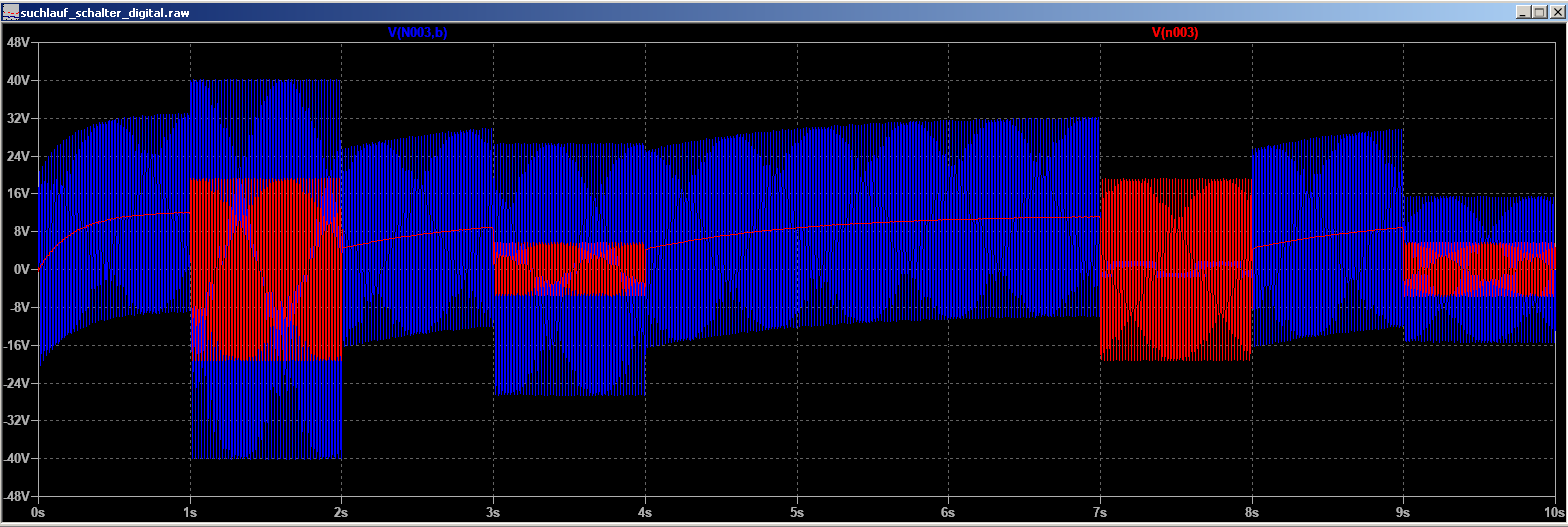
\includegraphics[width=\textwidth]{messen.png}};
\end{tikzpicture}
\caption{Spannung Rot: Suchlaufleitung -- AC 0V, Blau: Suchlaufleitung -- AC 15V -90°} \label{fig:1}
\end{figure}






\section{Aufbau} \label{sec:aufbau}

Die Schaltung wird auf zwei Platinen aufgebaut:
\begin{itemize}
\item Anschlussstecker Radio
\item Webradio
\end{itemize}

Die beiden Platinen werden "uber 2,54\,mm Stecker miteinander verbunden. Dies erm"oglicht ein leichtes Anpassen des Steckers auf Ger"atetypen mit anderer Buchse.


5v nie ohne ESP32, sonst VLSI hei"s -> kaputt.


\section{Inbetriebnahme} \label{sec:inbetriebnahme}


\subsection{OP / Comparatoren} \label{sec:op-cmp}

Versorgungsspannung 2x16\,V AC -- +/-22\,V. Die Comparatoren sind auf eine Versorgungsspannung von 22\,V berechnet. Da in der Schaltung Spannungsverh"altnisse verglichen werden sind die berechneten Schaltschwellen nur bei dieser Spannung g"ultig. Bei anderen Versorgungsspannungen verschieben sich die Schaltpunkte proportional zur Versorgungsspannung.

Alle Messungen mit Bezug auf die Mittelanzapfung der 15\,V Wicklung, nicht Masse des Radios!

\begin{figure}[H]
\centering
\begin{tikzpicture}
     \node[anchor=south west,inner sep=0] at (0,0) {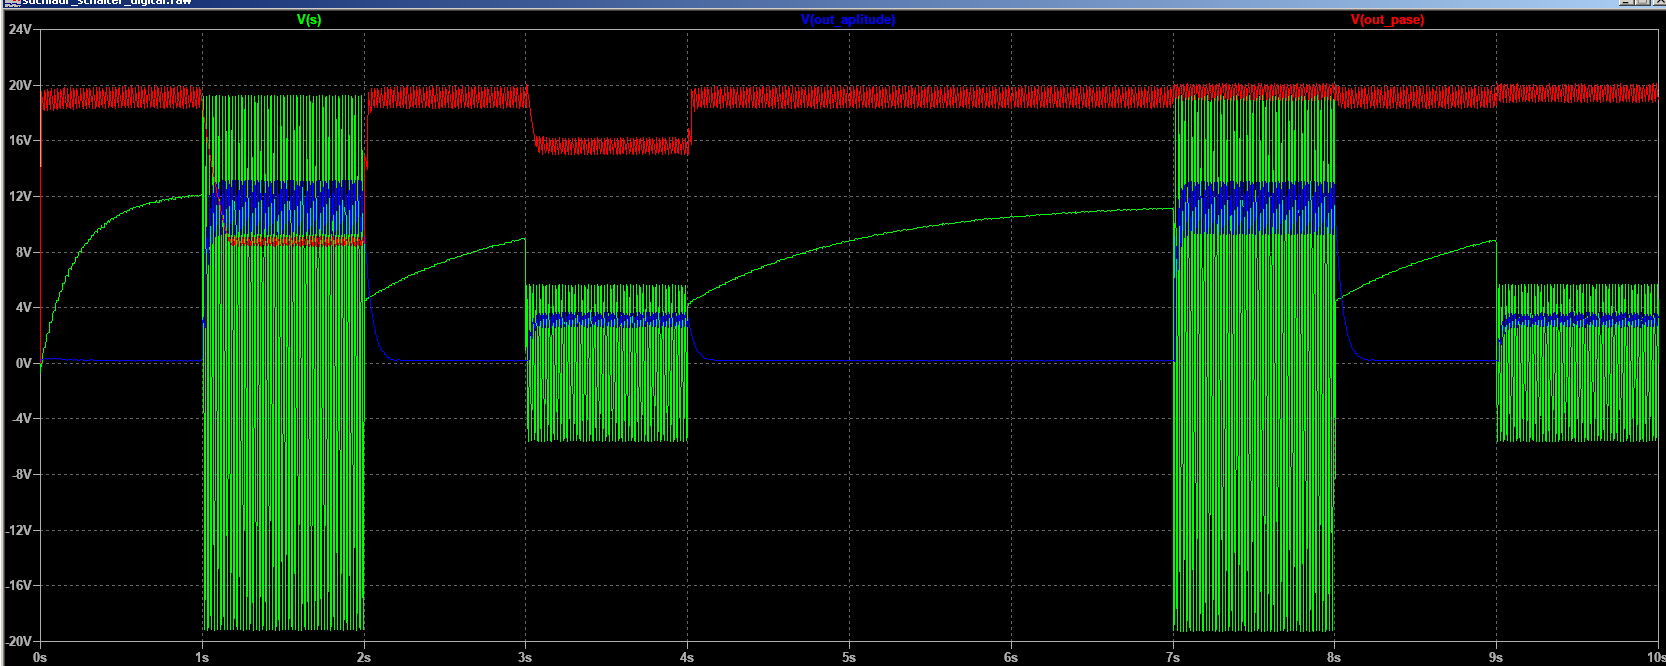
\includegraphics[width=\textwidth]{messen2.png}};
\end{tikzpicture}
\caption{Spannungen in Simulation} \label{fig:1}
\end{figure}

\textbf{Laufrichtung}

\begin{figure}[H]
\centering
\begin{tikzpicture}
     \node[anchor=south west,inner sep=0] at (0,0) {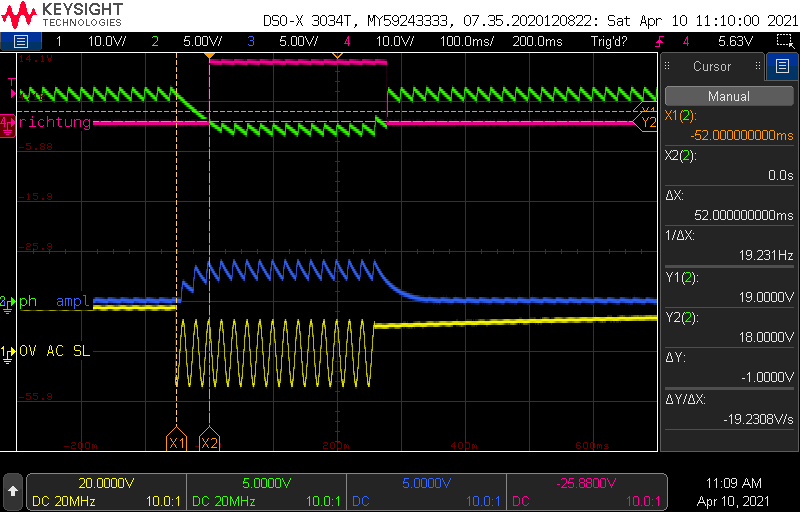
\includegraphics[width=\tscopesize]{image27346.png}};
\end{tikzpicture}
\caption{Laufrichtung 1, suchen} \label{fig:1}
\end{figure}

\begin{figure}[H]
\centering
\begin{tikzpicture}
     \node[anchor=south west,inner sep=0] at (0,0) {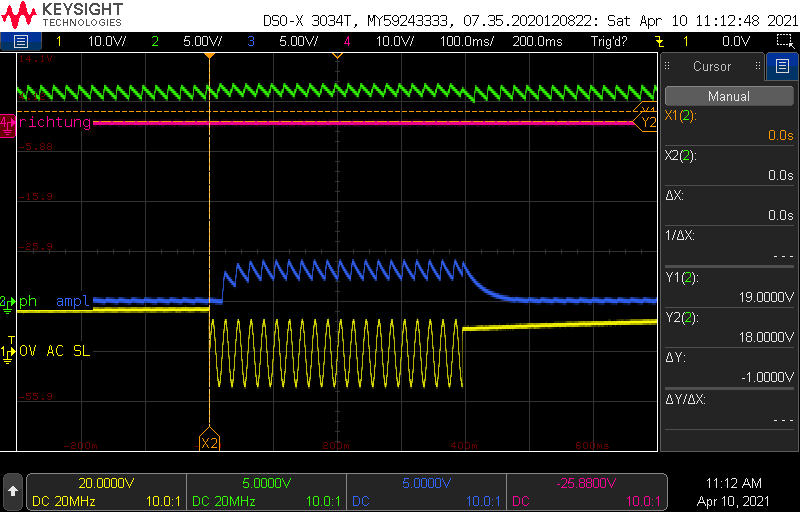
\includegraphics[width=\tscopesize]{image17823.png}};
\end{tikzpicture}
\caption{Laufrichtung 2, suchen} \label{fig:1}
\end{figure}

\begin{figure}[H]
\centering
\begin{tikzpicture}
     \node[anchor=south west,inner sep=0] at (0,0) {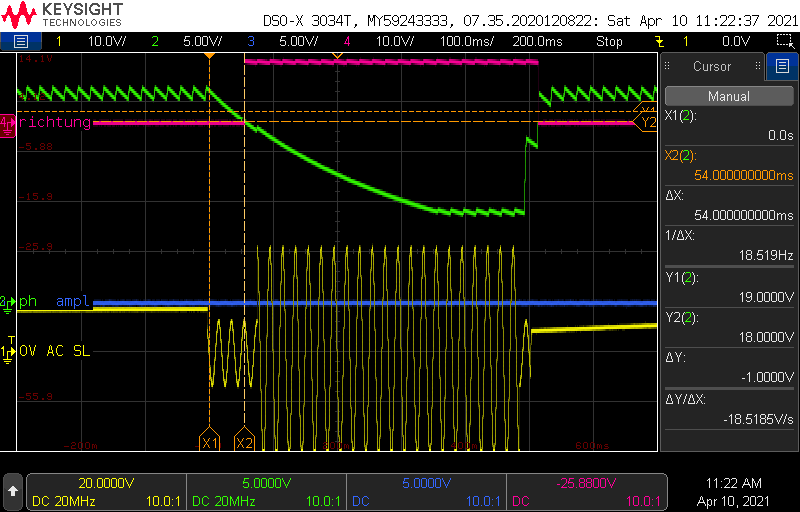
\includegraphics[width=\tscopesize]{image9355.png}};
\end{tikzpicture}
\caption{Laufrichtung 1, schnell} \label{fig:1}
\end{figure}

\begin{figure}[H]
\centering
\begin{tikzpicture}
     \node[anchor=south west,inner sep=0] at (0,0) {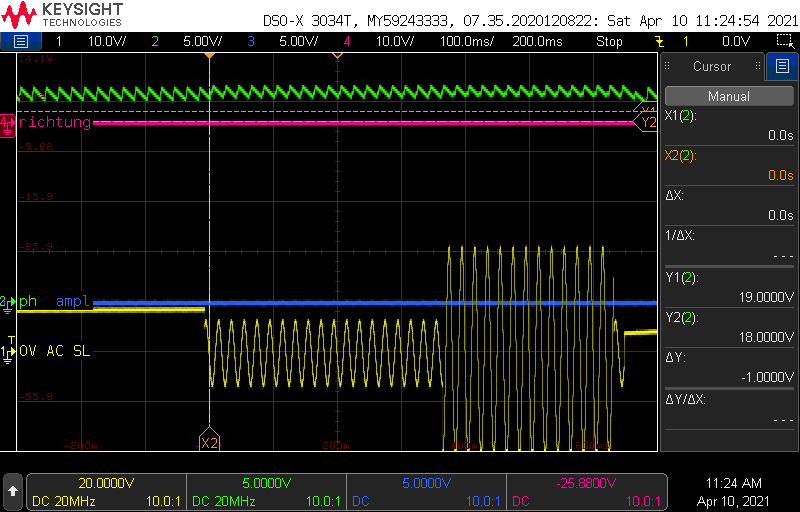
\includegraphics[width=\tscopesize]{image29704.png}};
\end{tikzpicture}
\caption{Laufrichtung 2, schnell} \label{fig:1}
\end{figure}

Die Laufrichtung wird korrekt erkannt. Die Spannungen sind wie erwartet. Die Verz"ogerung ist mit max. ca 50\,ms in einem akzeptablen Rahmen.

\textbf{Versorgungsspannung Laufrichtung}

Sweep Versorgungsspannung +/- 10\,V ... 18\,V AC. 

\begin{figure}[H]
\centering
\begin{tikzpicture}
     \node[anchor=south west,inner sep=0] at (0,0) {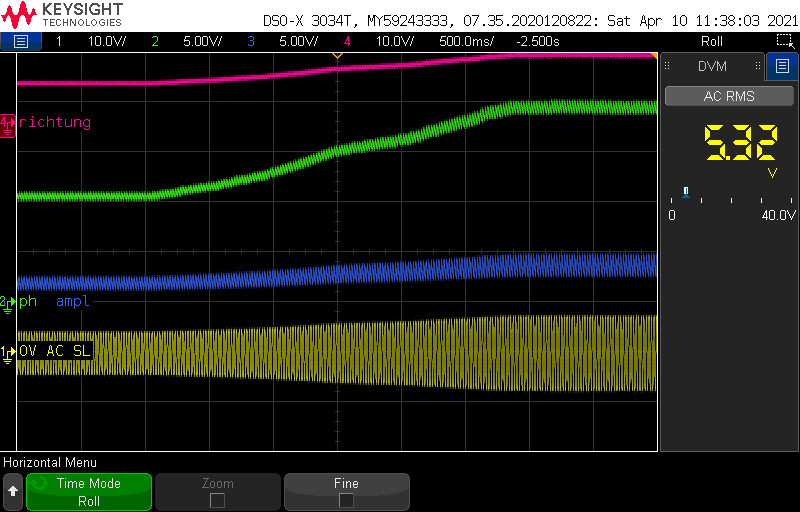
\includegraphics[width=\tscopesize]{image22258.png}};
\end{tikzpicture}
\caption{Laufrichtung 1, suchen} \label{fig:1}
\end{figure}

Das digitale Signal steht im gesamten Versorgungsspannungsbereich korrekt an. 

\todo wie wirken sich Widerstandstoleranzen des Teilers aus?

\textbf{Amplitude}

\begin{figure}[H]
\centering
\begin{tikzpicture}
     \node[anchor=south west,inner sep=0] at (0,0) {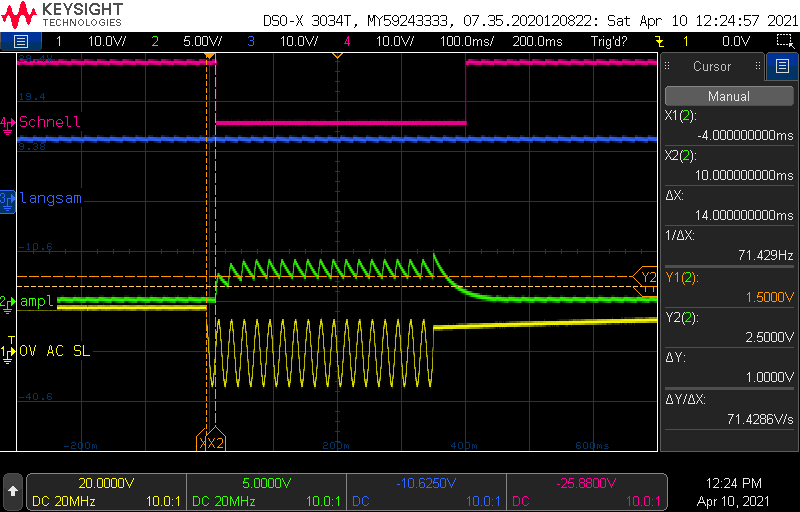
\includegraphics[width=\tscopesize]{image24190.png}};
\end{tikzpicture}
\caption{suchen} \label{fig:1}
\end{figure}

\begin{figure}[H]
\centering
\begin{tikzpicture}
     \node[anchor=south west,inner sep=0] at (0,0) {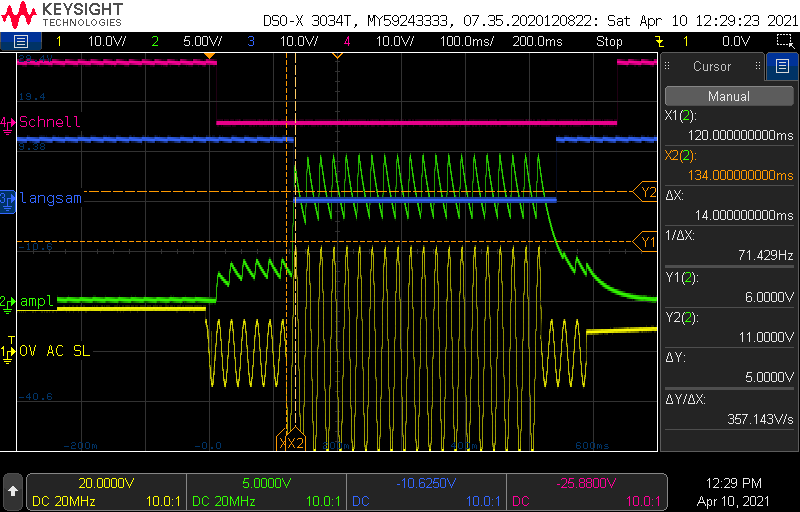
\includegraphics[width=\tscopesize]{image9293.png}};
\end{tikzpicture}
\caption{schnelllauf} \label{fig:1}
\end{figure}

Die Aplitude wird korrekt erkannt. Die Spannungen sind wie erwartet. Die Verz"ogerung ist mit max. ca 50\,ms in einem akzeptablen Rahmen.

\textbf{Versorgungsspannung Amplitude}

Sweep Versorgungsspannung +/- 10\,V ... 18\,V AC. 

\begin{figure}[H]
\centering
\begin{tikzpicture}
     \node[anchor=south west,inner sep=0] at (0,0) {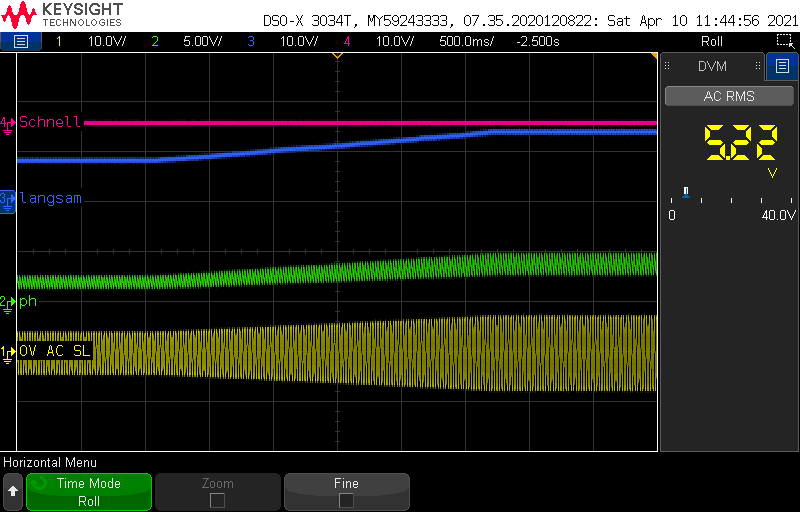
\includegraphics[width=\tscopesize]{image22512.png}};
\end{tikzpicture}
\caption{suchen} \label{fig:1}
\end{figure}

\begin{figure}[H]
\centering
\begin{tikzpicture}
     \node[anchor=south west,inner sep=0] at (0,0) {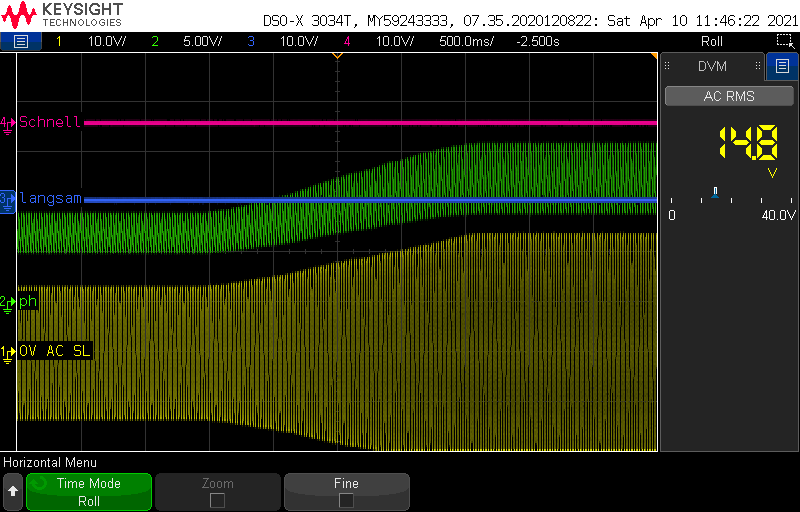
\includegraphics[width=\tscopesize]{image9576.png}};
\end{tikzpicture}
\caption{schnelllauf} \label{fig:1}
\end{figure}

Das digitale Signal steht im gesamten Versorgungsspannungsbereich korrekt an. 

\todo wie wirken sich Widerstandstoleranzen des Teilers aus?

\textbf{Amplitude}


\end{document}








